\chapter{Caso práctico}\label{cap:09caso}
En este capítulo se divide en cinco secciones: \ref{sec:09intro} Introducción, \ref{sec:09huvr} Estudio realizado por el HUVR, \ref{sec:09atlas} Estandarización del estudio con ATLAS, \ref{sec:09resultados} Discusión de resultados y \ref{sec:09conclusiones} Conclusiones.

\section{Introducción} \label{sec:09intro}

Este capítulo pretende demostrar la relevancia de OHDSI (Observational Health Data Science and Informatics) y la utilidad de sus herramientas, concretamente el uso de ATLAS para la estandarización y reproducibilidad de los análisis clínicos observacionales sobre bases de datos estandarizadas al Modelo de Datos Común de OMOP. 

Para ello, bajo la tutela de D. Carlos Parra y Da. Silvia Rodríguez (tutores de las prácticas en empresa, véase \ref{sec:03Participantes} ''Participantes del proyecto''), se ha seguido la reproducción de un estudio realizado por investigadores del hospital sobre predicción mediante modelos de ML de efectos adversos en el tratamiento radioterápico de pacientes con cáncer de pulmón. 

Este estudio, se encuentra públicamente accesible en Pubmed en dos artículos, el primero publicado en el año 2019 titulado \textit{''Comparison of Feature Selection Methods for Predicting RT-Induced Toxicity'' }\parencite{nunez2019comparison} y el segundo, en 2023 titulado \textbf{\textit{''Benchmarking machine learning approaches to predict radiation-induced toxicities in lung cancer patients''}} \parencite{nunez2023benchmarking}. Ambos estudios están también publicados en la ruta \code{Thesis-ATLAS-OHDSI/docs/pdf/estudioHUVR} del repositorio de github del TFG \parencite{vallealonsodc}.

El objetivo es promover el uso de ATLAS para la investigación observacional, reproduciendo mediante ATLAS un estudio que fue realizado sin hacer uso de la herramienta, para demostrar con un caso práctico los beneficios de utilizar la herramienta en términos de reproducibilidad y estandarización.

\section{Estudio realizado por el HUVR} \label{sec:09huvr}

El estudio consiste en la comparación de 300 modelos de ML sobre un dataset de 875 pacientes de cancer de pulmón con el objetivo de predecir los efectos adversos a corto (esofagitis, tos, disnea y neumonitis) y a largo plazo (disnea y neumonitis) que producirá el tratamiento radioterápico sobre estos pacientes. 

\subsubsection{Contexto}

%La base teórica del estudio \parencite{nunez2019comparison, nunez2023benchmarking} es que la radioterapia aunque es beneficiosa para el tratamiento oncológico, también causa efectos perjudiciales a corto y/o  largo plazo de forma personalizada según las condiciones de cada paciente. El auge de la medicina personalizada y centrada en el paciente (véase \ref{sec:01Contexto}) ha ensalzado la importancia de realizar una planificación individual para cada paciente, pues cada persona responde de forma distinta a los tratamientos. Por tanto, la gestión individualizada de los posibles efectos adversos es muy importante en la planificación del tratamiento radioterápico, con el fin de facilitar la toma de decisiones entre médico y paciente en términos de calidad de vida y posibilidades de supervivencia.

La radioterapia, aunque beneficia el tratamiento oncológico, puede ocasionar efectos perjudiciales a corto y largo plazo, de forma personalizada según cada paciente \parencite{nunez2019comparison, nunez2023benchmarking}. La medicina centrada en el paciente (véase \ref{sec:01Contexto} ''Marco contextual'') destaca la importancia de planificar individualmente cada tratamiento, dado que las respuestas varían entre individuos. Por tanto, la gestión personalizada de los efectos adversos es crucial en la planificación radioterápica para facilitar la toma de decisiones médico-paciente en términos de calidad de vida y supervivencia.

\subsubsection{Objetivo}

El objetivo del estudio es utilizar un conjunto de datos del mundo real (RWD) para facilitar la toma de decisiones clínicas, estudiando para cada efecto adverso del tratamiento radioterápico, el modelo de ML que provee una mejor predicción en términos de precisión del modelo (AUC).

\subsubsection{Datos}

El estudio utiliza datos del mundo real (RWHD) obtenidos de la combinación entre los datos almacenados en el registro S31 del HUVR y otros datos recogidos en consultas oncológicas rutinarias del hospital. La descripción de los datos del registro S31 se encuentra en el apéndice A del artículo ''Benchmarking machine learning approaches to predict radiation-induced toxicities in lung cancer patients'', también disponible en la ruta del repositorio de github \code{Thesis-ATLAS-OHDSI/docs/pdf/estudioHUVR/appendixA.pdf}.

En resumen los datos consisten en una recopilación de pacientes de cáncer de pulmón, con datos concológicos descriptivos, datos de los tratamientos recibidos por el paciente  y los efectos adversos sufridos.

\subsubsection{Metodología}

Para conformar los 300 modelos de ML se han entrenado y testeado 5 modelos de ML combinados con 10 métodos de selección de atributos (\textit{Feature Selection, FS}) sobre 6 efectos adversos (\textit{outcomes} o \textit{clinical endpoints}), de la siguiente forma: 

\begin{itemize}
    \item \textbf{5 Modelos de ML}. Se utilizaron cinco clasificadores basados en aprendizaje 
    automático: 
    \begin{itemize}[label={--}]
        \item Máquina de Vectores de Soporte (\textit{Support Vector Machine, SVM}).
        \item Vecinos más Cercanos (\textit{k-Nearest Neighborhood, kNN}).
        \item Red Neuronal Artificial (\textit{Artificial, Neural Network, ANN}) de alimentación directa.
        \item Modelo Lineal Generalizado (\textit{Generalized Linear Model, GLM}).
        \item Clasificador de Naïve-Bayes (\textit{NB}).
    \end{itemize}
     Los hiperparámetros de los modelos se se optimizaron automáticamente siguiendo ''las recomendaciones de la literatura''.
    
    \item \textbf{10 Métodos de Selección de Atributos \textit{(FS)}.} Para reducir la dimensionalidad de los conjuntos de datos, se implementaron los siguientes métodos:
    
    \begin{itemize}[label={--}]
        \item Selección de Características Basada en Correlación (\textit{Correlation-based Feature Selection, CFS}).
        \item Chi-cuadrado %(\( \chi^2 \)).
        \item Boruta.
        \item Mínima Redundancia - Máxima Relevancia (\textit{Minimum Redundancy-Maximum Relevance, mRMR}).
        \item Relief.
        \item Ganancia de Información (\textit{Information Gain, IG}).
        \item  Bosque Aleatorio (\textit{Random Forest, RF}).
        \item 2 métodos de ensamblaje a partir de métodos de FS individuales y de subconjuntos.
        \item Subconjuntos de variables determinadas por un oncólogo experto para predecir las toxicidades seleccionadas basadas en la evidencia clínica.
    \end{itemize}

    \item \textbf{6 Efectos adversos.} Se seleccionaron seis efectos adveros a estudiar, clasificados según si su duración fue a corto plazo y a largo plazo. A corto plazo:
    \begin{itemize}[label={--}]
        \item Esofagitis.
        \item Tos.
        \item Disnea. 
        \item Neumonitis. 
    \end{itemize}
    A largo plazo:
    \begin{itemize}[label={--}]
        \item Disnea. 
        \item Neumonitis. 
    \end{itemize}
    Se consideran efectos adversos crónicos o a largo plazo si los efectos se mantuvieron presente más de tres meses a partir del inicio del tratamiento.
\end{itemize}

Para la validación interna de los modelos se ha utilizado una estrategia de validación cruzada de 10 pliegues (\textit{10-fold Cross-Validation}) en la que se aplicó una técnica de submuestreo aleatorio para generar un conjunto de datos equilibrado. Para la validación externa, se han utilizado los datos generados con los casos registrados después del 31 de mayo de 2018, que no fueron utilizados para la validación interna. 

Por último, el rendimiento de los modelos se ha medido en términos del AUC logrado por cada modelo predictivo.

\subsubsection{Resultados}

   Los resultados del estudio resaltan para cada outcome el mejor modelo de ML y selección de atributos, con la valoración de AUC en validación interna y externa. Los resultados se muestran de forma muy intuitiva en la siguiente tabla, extraída del artículo del HUVR \parencite{nunez2023benchmarking}.

\begin{figure}[H]
    \centering
    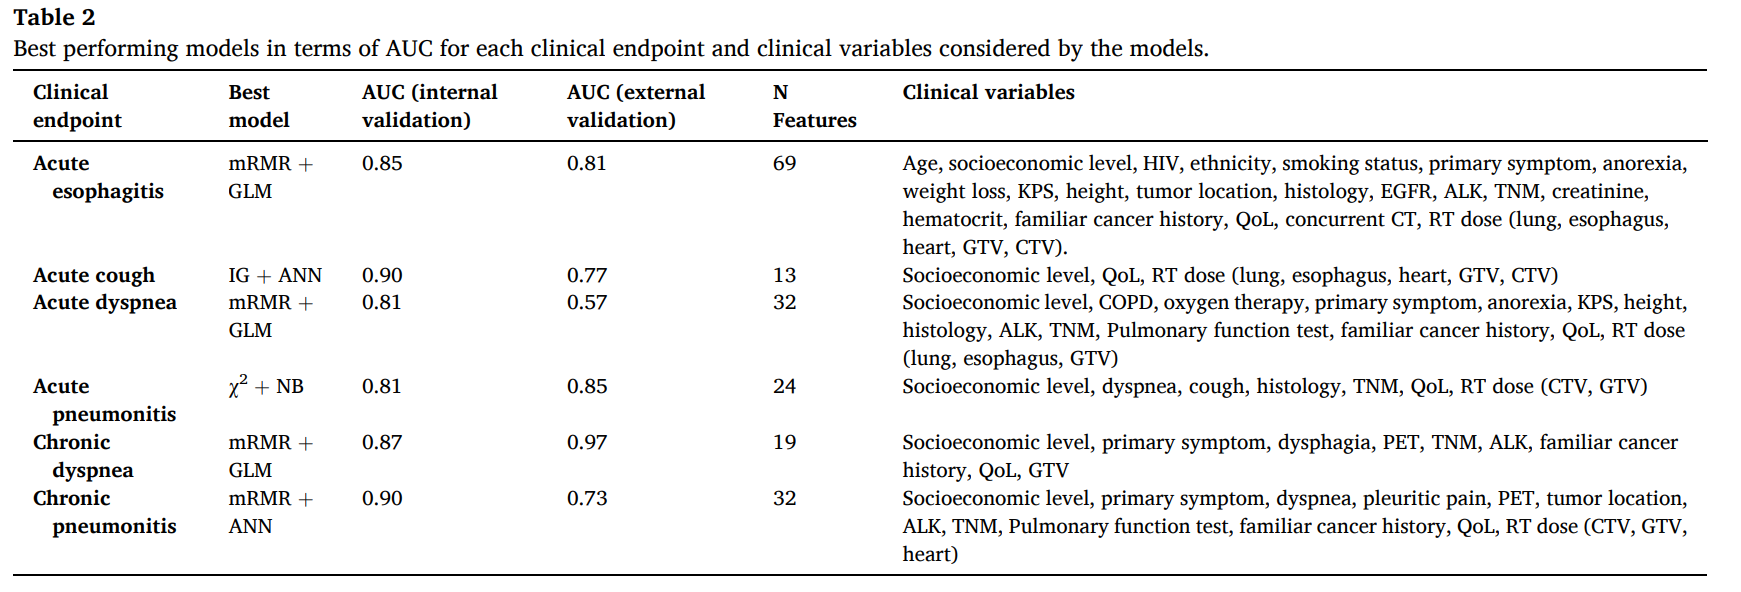
\includegraphics[width=1\textwidth]{tables/nune2023table2.png}
    \captionof{table}{Recopilación de resultados del estudio del HUVR. Extraída de \parencite{nunez2023benchmarking}}
    \label{table:nune2023table2}
\end{figure}


\section{Estandarización del estudio con ATLAS} \label{sec:09atlas}

Este capítulo presenta el caso práctico realizado por la alumna en el que se aplican todos los contenidos teóricos y herramientas presentadas a lo largo de la memoria para realizar un análisis de datos real.

%\subsubsection{Objetivo}

\textbf{El objetivo de este estudio se alinea con el objetivo de OHDSI: estandarizar la investigación clínica observacional}, mediante el Modelo de Datos Común de OMOP y la herramienta de análisis de datos ATLAS. No se pretende meramente reproducir el estudio haciendo uso del ecosistema de OHDSI sino que se destaca que el fin último del proyecto es estandarizar el estudio, adaptarlo al marco de investigación OHDSI para que cualquier nodo de la organización pudiera procesarlo, analizarlo y reproducirlo fácilmente. 

%\subsubsection{Ádaptación del estudio al marco de OHDSI}

\textbf{En el marco de OHDSI, el estudio realizado por el HUVR  corresponde al caso de uso de Predicción a nivel de Paciente} (recuerde \ref{subsec:05casosUso} ''Casos de uso para la investigación''). Tiene el objetivo de construir modelos que predigan la probabilidad de experimentar un efecto concreto en función de las características concretas de los pacientes. 

No obstante, para poder aplicar en el análisis con ATLAS los otros dos casos de uso estudiados (Caracterización y Estimación a Nivel de Población ), se ha adaptado el estudio bajo las consideraciones necesarias para que tuviera sentido. Por ello, la finalidad del caso práctico no es una reproducción fiel del estudio sino la estandarización del estudio al marco de investigación metodológica de OHDSI.

%\textbf{El objetivo es demostrar la reproducibilidad de cualquier estudio adaptándolo al marco de investigación OHDSI} y, por tanto, estandarizándolo a una metodología de investigación concreta que facilite aún más su reproducibilidad a nivel global. Una vez que la base de datos se encuentre omopizada y se realice el análisis con ATLAS, el estudio se podrá replicar fácilmente en cualquier lugar del mundo, en cualquier nodo de la red de OHDSI, tal y como se mostró en el ''ejemplo de la plancha'' (véase \ref{subsec:05caracteristicas} ''Características de la organización''). 


\subsection{Datos}
%\subsection{Comprobación calidad datos}

En cuanto a los datos empleados, se ha utilizado una base de datos montada por el equipo de investigadores del HUVR en un servidor PostgreSQL

La estructura original de la base de datos proporcionada no correspondía con el Modelo de Datos Común de OMOP por lo que una tarea crucial de preprocesamiento ha sido el \textbf{OMOPizado de la base de datos y la comprobación de calidad de los datos}, realizado por mi compañero Francisco Rey Garduño como objeto de su Trabajo de Fin de Grado ''Análisis de datos sanitarios mediante herramientas OHDSI y modelo de datos OMOP''.

Por otra parte, es importante destacar que \textbf{la base de datos que se ha utilizado no es exactamente igual a la del estudio original} debido a motivos internos del equipo de investigación. La base de datos utilizada es una combinación y adaptación entre los datos del registro S31 y S32 del HUVR con una modificación importante: no incluye las variables relacionadas con las toxicidades experimentadas por los pacientes. Por tanto, las partes del estudio que involucran estas variables solo serán diseñadas pero no probadas en la herramienta.

\subsection{Metodología}

El estudio se ha realizado utilizando la herramienta ATLAS Broadsea. A estas alturas se conoce que el componente central de los estudios observacionales en OHDSI es el estudio de cohortes (recuerde \ref{subsec:05cohortes} ''Cohortes''). Según el caso de uso que se diseñe sobre la cohorte se obtiene un tipo de evidencia u otro. En este caso, se va a realizar un estudio de cada caso de uso, utilizando en la medida necesaria las configuraciones recomendadas por defecto que ofrece la herramienta.

\subsubsection{Análisis exploratorio}

En primer lugar, es interesante realizar un breve análisis exploratorio de la base de datos. Para ello la herramienta \code{Data Sources} de ATLAS proporciona una interfaz muy intuitiva para generar reportes automáticamente según las características más relevantes de la base de datos.

\begin{figure}[H]
    \centering
    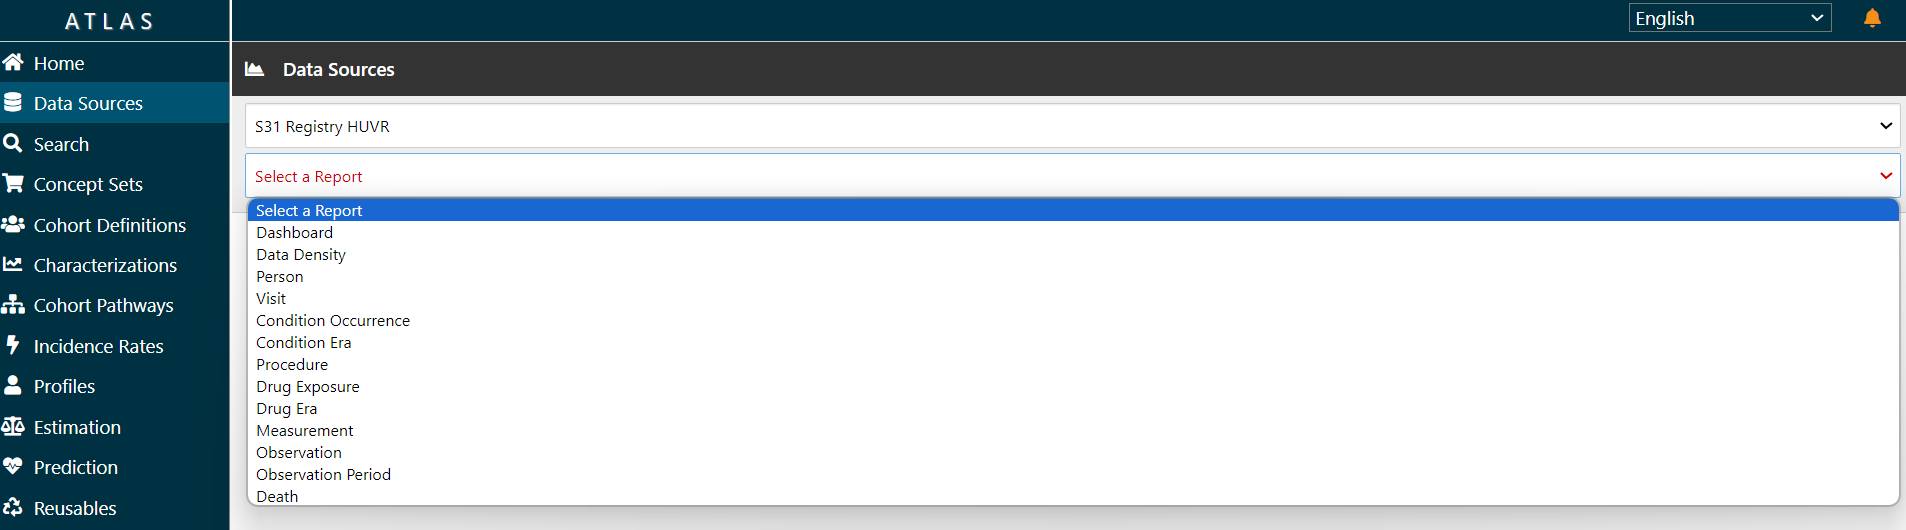
\includegraphics[width=1\textwidth]{figures/atlasDataSources.png}
    \caption{Seleccionador del reporte que se desea generar sobre sobre la base de datos S31/32 Registry HUVR}
    \label{figure:atlasDataSources}
\end{figure}


A continuación se adjuntan los gráficos más relevantes del conjunto total de reportes. Todos los gráficos del conjunto total de reportes se han descargado y subido al repositorio de github en la ruta \code{Thesis-ATLAS-OHDSI/atlas/reports}.

\begin{figure}[H]
    \centering
    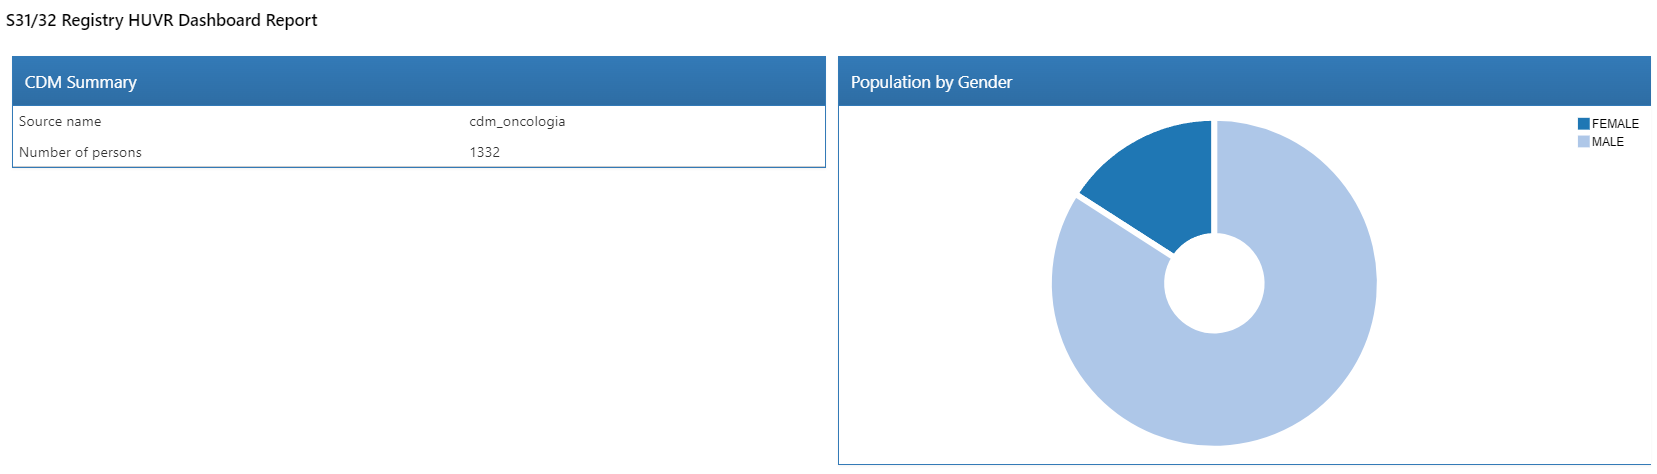
\includegraphics[width=1\textwidth]{figures/dashboardREPORT.png}
    \caption{Reporte general de la información de la base de datos S31/32 Registry HUVR}
    \label{figure:dashboardREPORT}
\end{figure}

La base de datos contiene 1332 registros de pacientes, es decir, un número mayor que la base de datos utilizadas en el estudio del HUVR. Esto se debe a que las bases de datos no son exactamente las mismas y la base de datos utilizada en el proyecto es una combinación del registro S31 y S32 procedente de la fuente original denominada \code{omop\_oncologia}. Por otra parte, el 84.1\% de la población registrada es masculina y el 15.9\% es femenina.

\begin{figure}[H]
    \centering
    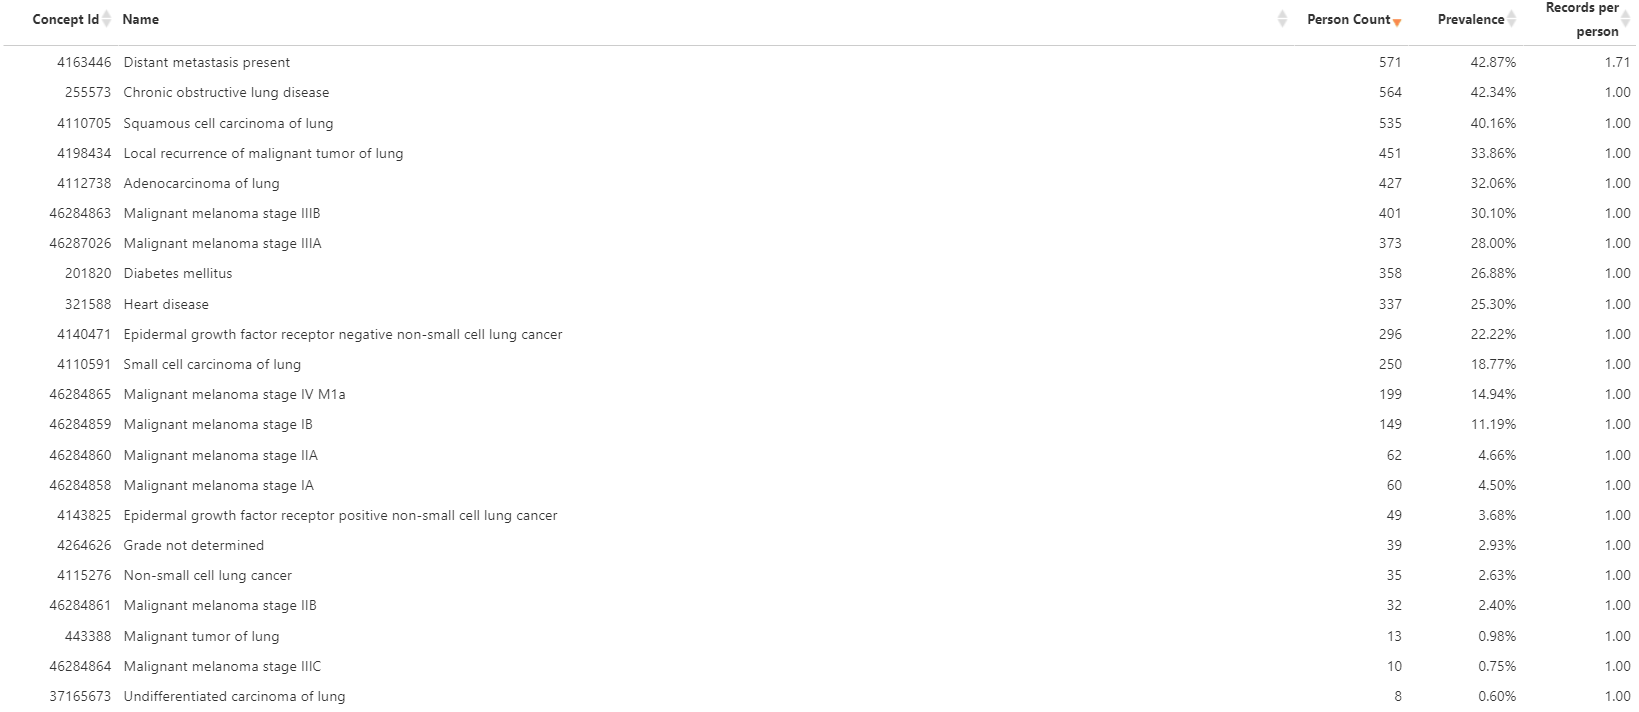
\includegraphics[width=1\textwidth]{tables/conditionOcurrenceREPORT.png}
    \captionof{table}{Reporte de las condiciones registradas en la base de datos S31/32 Registry HUVR}
    \label{table:conditionOcurrenceREPORT}
\end{figure}

Las condiciones registradas en la base de datos son mayoritariamente conceptos distintos que describen distintas características del cáncer de pulmón. Estos conceptos posteriormente se agruparán en un único grupo de concepto para facilitar el estudio. También aparecen las condiciones de diabetes mellitus y enfermedad cardíaca, aunque estas no son muy relevantes para el estudio.

Es importante recordar que no aparece en el reporte ningún tipo de condición relacionada con alguno de los efectos adversos identificados en el estudio original (disnea aguda, disnea crónica, neumonitis aguda, neumonitis crónica, esofagitis o tos) debido a que no están incluidos en la base de datos facilitada por el HUVR.

\begin{figure}[H]
    \centering
    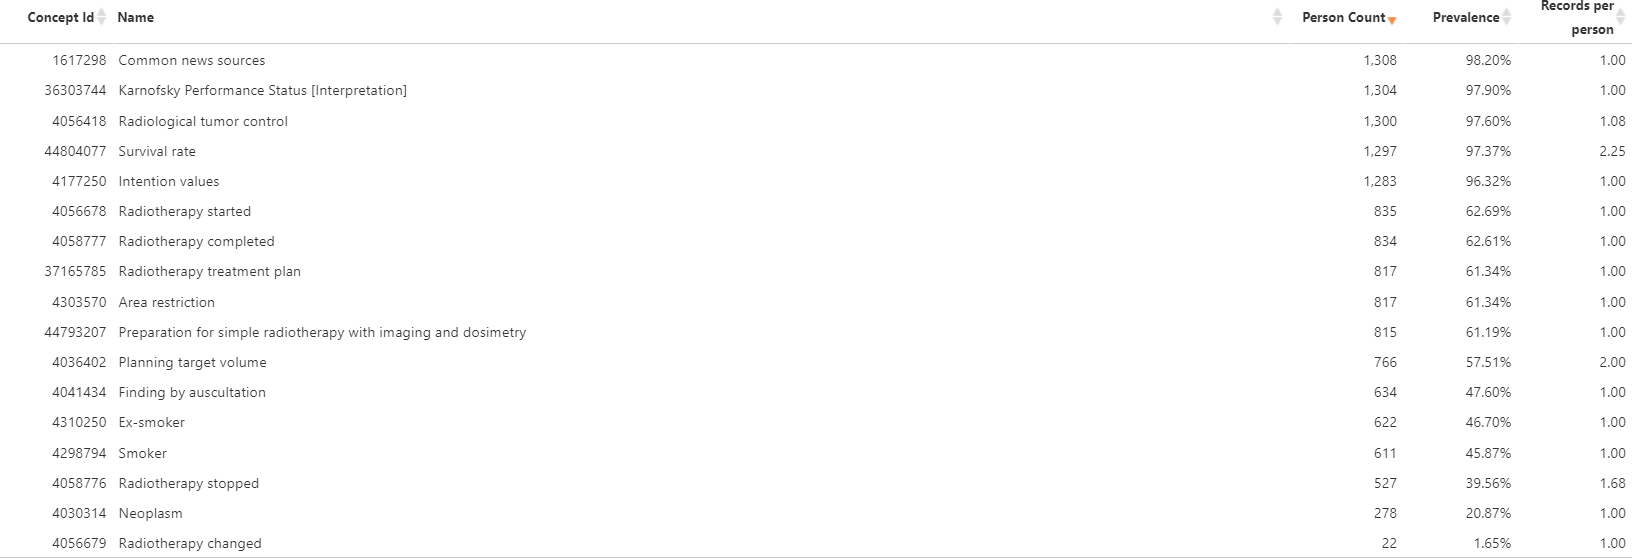
\includegraphics[width=1\textwidth]{tables/observationREPORT.png}
    \captionof{table}{Reporte de las observaciones registradas en la base de datos S31/32 Registry HUVR}
    \label{figure:observationREPORT}
\end{figure}

Las observaciones registradas en la base de datos hacen referencia a características observables en el paciente. Las observaciones más destacables son aquellas relacionadas con la planificación del tratamiento radioterápico.

\begin{figure}[H]
    \centering
    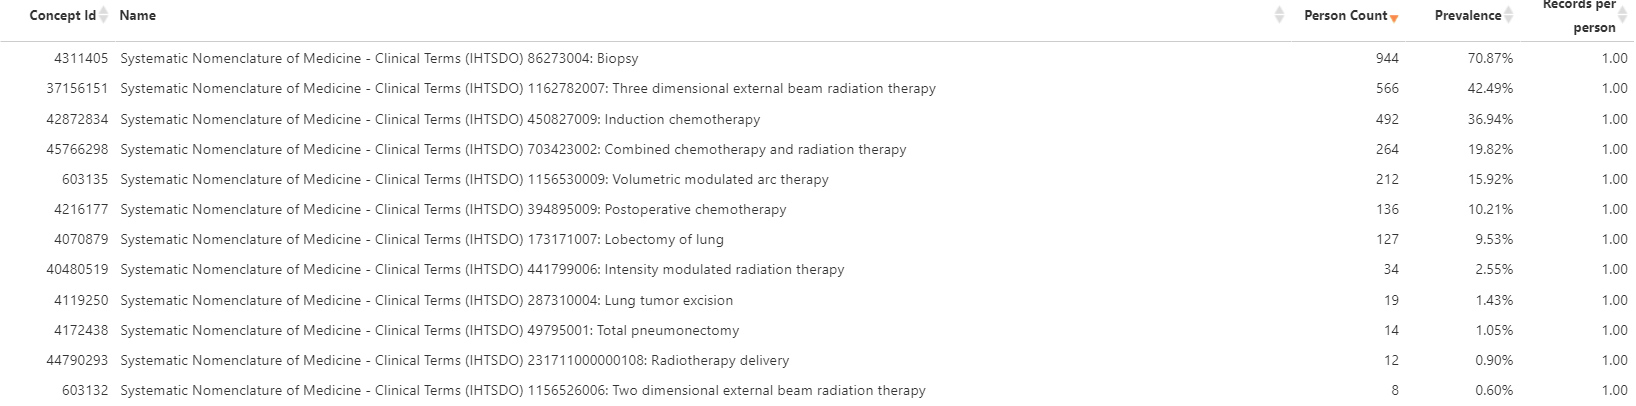
\includegraphics[width=1\textwidth]{tables/procedureREPORT.png}
    \captionof{table}{Reporte de los procedimientos registrados en la base de datos S31/32 Registry HUVR}
    \label{table:procedureREPORT}
\end{figure}

Los procedimientos registrados en la base de datos presentan una característica común y es que todos están mapeados a SNOMED CT, el estándar por excelencia para definir este tipo de información. Los procedimientos se pueden agrupar en tres conjuntos: radioterapia, quimioterapia y cirugía torácica. Estos tres conjuntos formarán a continuación otros tres grupos de conceptos.

\subsubsection{Grupos de Conceptos}

Una vez se conocen los conceptos más relevantes en el estudio, estos se puede asociar en grupos según los eventos clínicos a los que hacen referencia, tal y como se sugiría en el apartado anterior. Esta tarea se realiza a través del menú \code{Concept Sets} de ATLAS.

Se han identificado y definido 12 grupos de conceptos relevantes en el estudio. A continuación se muestra el listado de los grupos de conceptos empleados en el estudio.

\begin{figure}[H]
    \centering
    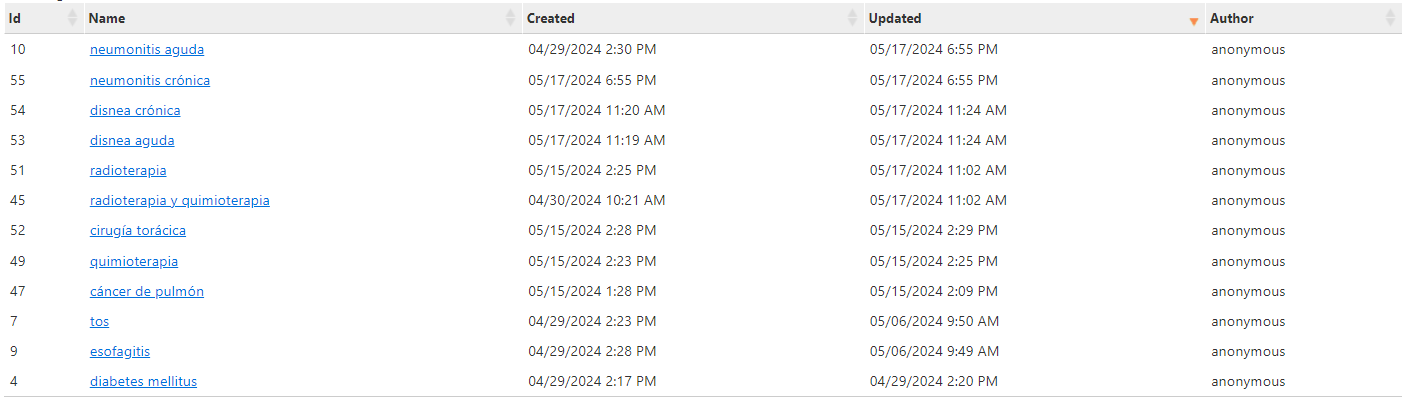
\includegraphics[width=1\textwidth]{tables/conceptSetLIST.png}
    \captionof{table}{Listado de los 12 grupos de conceptos definidos en ATLAS Broadsea}
    \label{table:conceptSetLIST}
\end{figure}

Los grupos de conceptos se pueden clasificar en tres temáticas según la utilidad que tienen en el estudio:

\begin{itemize}

    \item \textbf{Condición prevalente.} La condición que prevalece en las base de datos es el cáncer de pulmón (CP).
    \item \textbf{Tratamientos oncológicos.} El estudio distingue tres tipos de tratamiento oncológico: radioterapia (RT), quimioterapia (QT) y cirugía torácica (IQ).
    \item \textbf{Toxicidades inducidas.} El estudio identifica seis tipos de toxicidades inducidas: disnea aguda (DA), disnea crónica (DC), neumonitis aguda (NA), neumonitis crónica (NC), tos (T) y esofagitis (E).
    
\end{itemize}

En este caso, aunque la base de datos no contiene información sobre las toxicidades inducidas, mediante la búsqueda genérica en el vocabulario (a través de la herramienta \code{Search}) se han definido grupos de conceptos relacionados con estas variables. De este modo se pueden hacer presente y continuar diseñando el estudio aunque no tengan presencia real en la base de datos. 

La definición de cada grupo de concepto se ha exportado a archivos json y se encuentran accesibles en la ruta del repositorio de github \code{Thesis-ATLAS-OHDSI/atlas/concept sets}.

\subsubsection{Cohortes}

La definición de las cohortes es el componente central del estudio. Las cohortes son los componentes que luego combinándose entre sí y junto a otros parámetros conforman los distintos tipos de estudio (véase \ref{sec:05Evidencia} ''¿Cómo generar evidencia?''). La definición de cohortes se realiza a través del menú \code{Cohort Definitions} de ATLAS.

En el proyecto se han definido 14 cohortes combinando los grupos de conceptos definidos previamente.

\begin{figure}[H]
    \centering
    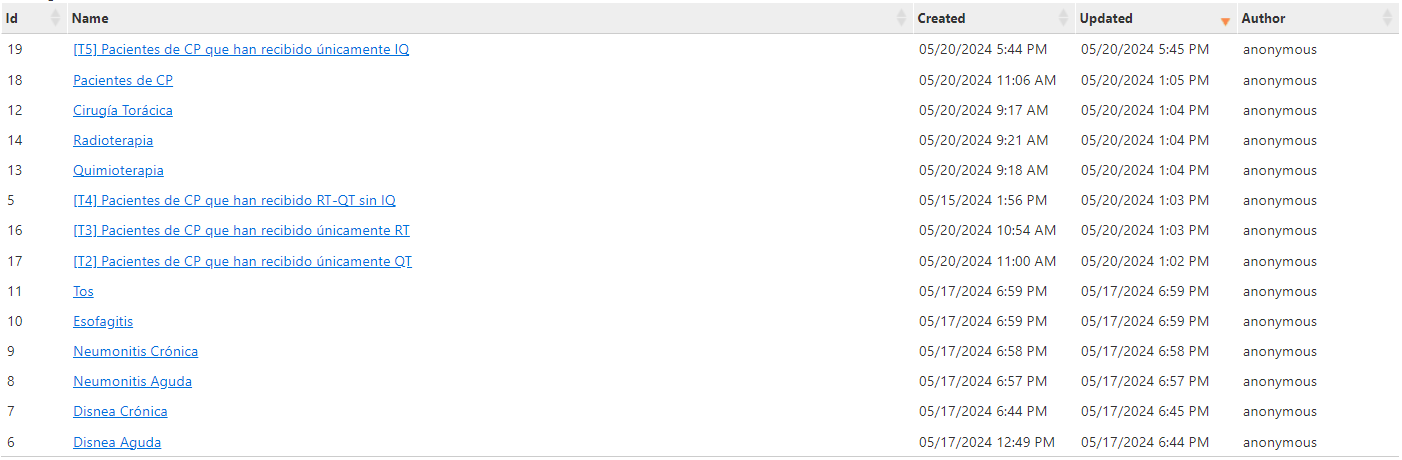
\includegraphics[width=1\textwidth]{tables/cohortLIST.png}
    \captionof{table}{Listado de las 14 cohortes definidas en ATLAS}
    \label{table:cohortLIST}
\end{figure}

Se puede observar que hay dos formas diferentes de definir las cohortes en función de la utilidad que tienen en el estudio:

\begin{itemize}

    \item \textbf{Cohorte principal \textit{(Target)}:} Este tipo de cohorte representa a la población sobre la que se realiza el estudio. Suelen ser poblaciones con características muy concretas y su definición incluye uno o varios criterios de inclusión más específicos.

    En el proyecto, las cohortes principales son las cuatro cohortes cuyo nombre empieza por [T] y la cohorte primitiva \code{Pacientes de CP}. Se le denomina cohorte primitiva porque es la cohorte genérica que no aplica ninguna restricción al conjunto de pacientes de cáncer de pulmón. Por otro lado, la etiqueta [T] en las cohortes es un identificador que la asocia con las cohortes definidas internamente en el estudio del HUVR. 

    \item \textbf{Cohorte de resultado \textit{(Outcome)}:} Este tipo de cohorte representa a la población que experimenta un \textit{outcome} o efecto adverso. Su definición es mucho más sencilla, simplemente representan la población que experimenta una condición concreta.
    
    Su función es servir de parámetro para configurar los estudios posteriores que se realizan sobre las cohorte principales.
 
\end{itemize}

La definición de las cohortes se ha exportado a archivos json y sql y se encuentran accesibles en la ruta del repositorio de github \code{Thesis-ATLAS-OHDSI/atlas/cohort definitions}.

\subsubsection{Caracterización}

Con esta sección comienza el primero de los casos de uso definidos para la investigación observacional de OHDSI. Aunque estrictamente la generación de reportes de la base de datos también se considera caracterización, esta sección se centra en la caracterización de cohortes.

Para ello se emplean dos herramientas de ATLAS: \code{Characterization} y \code{Cohort Pathway}.

La caracterización consiste en la obtención de un reporte con las características estadísticas más relevantes de la cohorte. 

En este caso se ha realizado una caracterización que compara tres cohortes principales del estudio: pacientes que han recibido únicamente quimioterapia, pacientes que han recibido únicamente radioterapia, y pacientes que han recibido ambas terapias sin sufrir cirugía torácica. Esta última cohorte es la que se utiliza para diseñar el resto de casos de uso de la investigación. 


\begin{figure}[H]
    \centering
    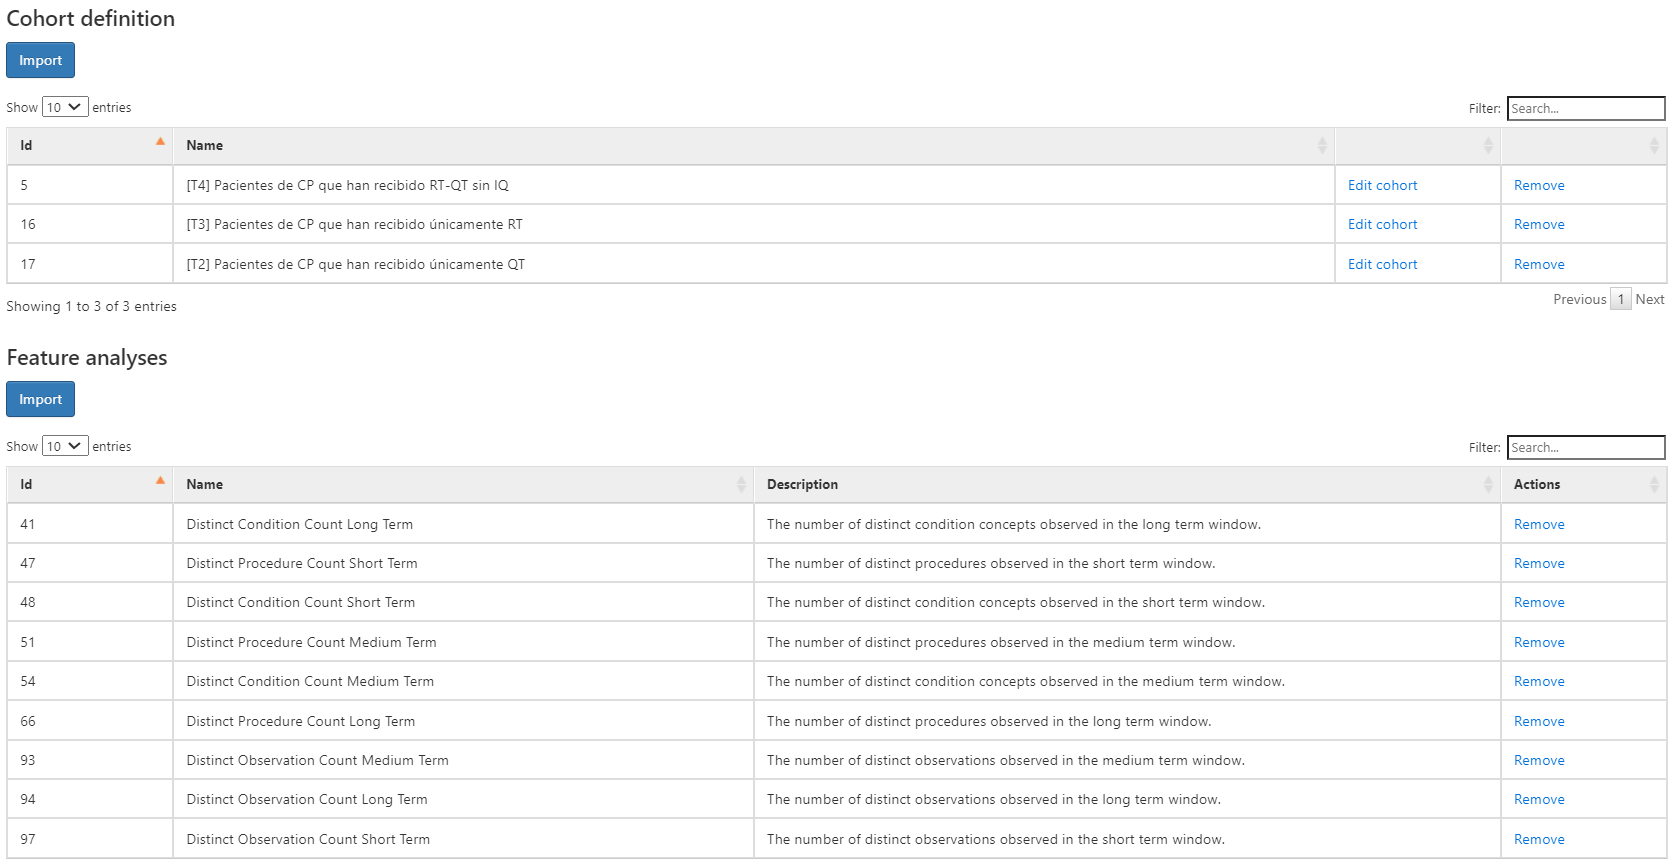
\includegraphics[width=1\textwidth]{tables/characterization_statistics.png}
    \captionof{table}{Definición del análisis estadístico de las cohortes principales}
    \label{table:characterization_statistics}
\end{figure}

Las variables seleccionadas para diseñar el estudio de caracterización han sido aquellas relacionadas con las distintas condiciones, procedimientos y observaciones que experimentan las cohortes.  Los resultados y el diseño del análisis se han exportado y están disponibles en la ruta del repositorio de github \code{Thesis-ATLAS-OHDSI/atlas/characterization 
 s/characterization\_1\_execution\_72\_reports}.

Otra forma de caracterizar una cohorte es a través de la ruta de la cohorte. En este caso se ha diseñado una ruta de la cohorte que estudie las diferentes rutas de tratamiento (quimioterapia, radioterapia y cirugía torácica) que experimenta la cohorte primitiva de cáncer de pulmón..

\begin{figure}[H]
    \centering
    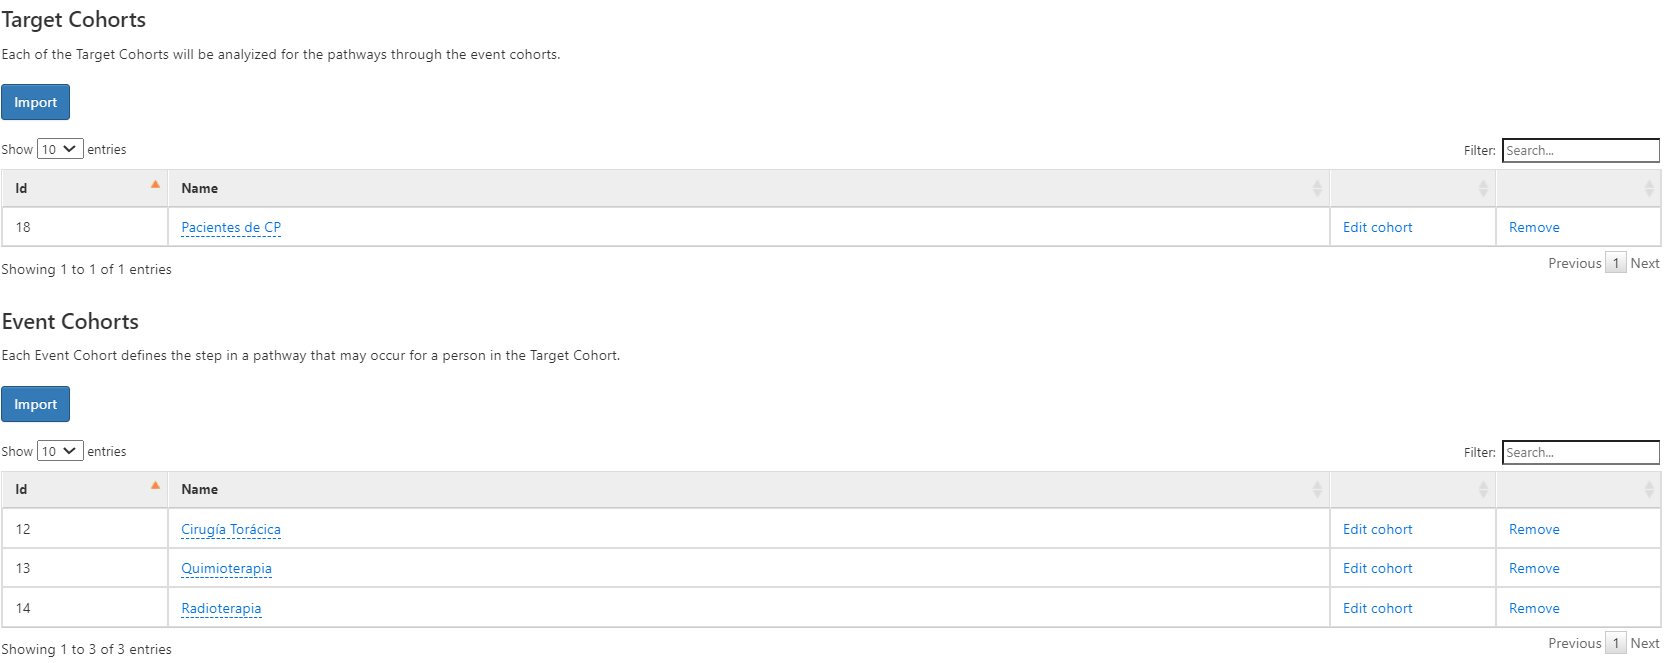
\includegraphics[width=1\textwidth]{tables/pathway_definition.png}
    \captionof{table}{Definición del análisis de la ruta de la cohorte de cáncer de pulmón}
    \label{table:pathway_definition}
\end{figure}

\begin{figure}[H]
    \centering
    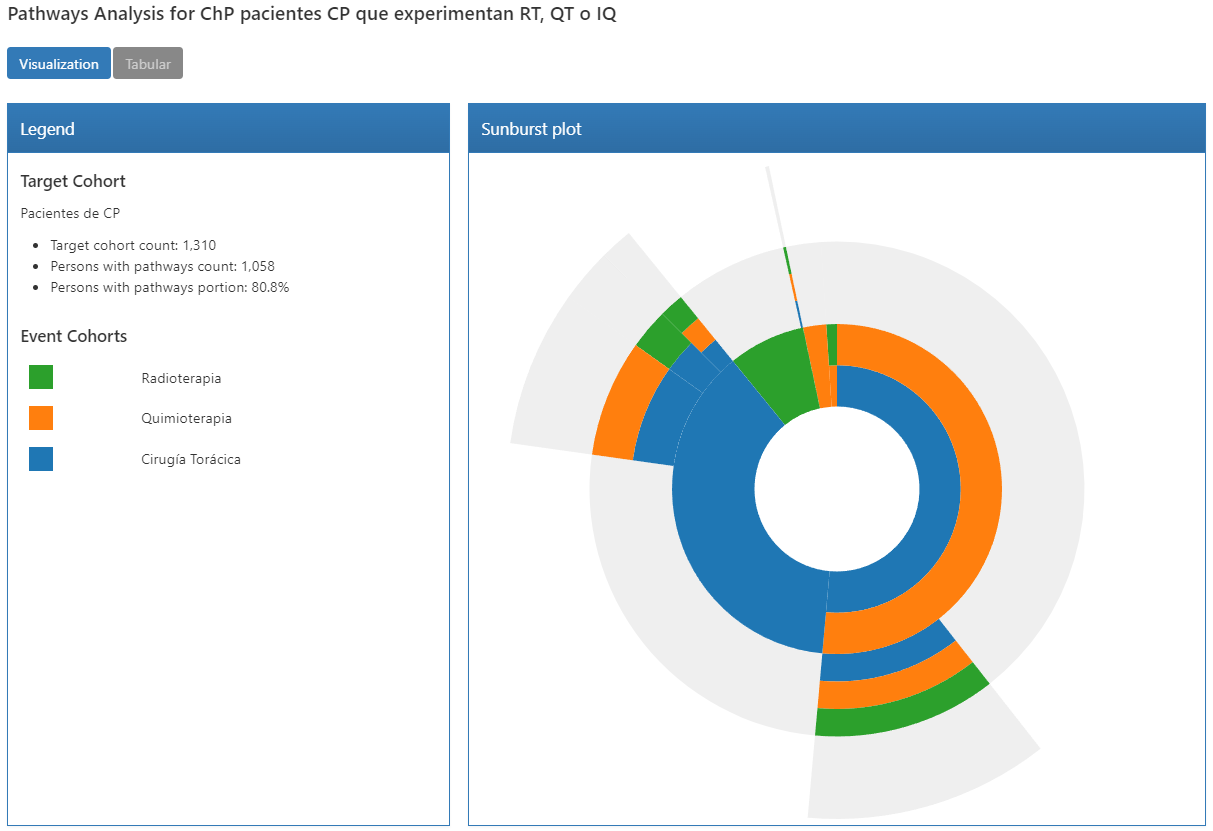
\includegraphics[width=1\textwidth]{figures/pathway.png}
    \caption{Análisis de las rutas de la cohorte de cáncer de pulmón}
    \label{table:pathway}
\end{figure}

En este caso, el resultado se muestra en la Figura \ref{table:pathway} que se obtiene es una ''gráfica de explosión solar'' o \textit{surnbust} que muestra las diferentes rutas que experimenta la cohorte. No obstante, tanto la definición del estudio como los resultados también se encuentran accesibles a través de la ruta del repositorio de github \code{Thesis-ATLAS-OHDSI/atlas/characterizations/cohort pathway} 


\subsubsection{Estimación a Nivel Población}

La estimación a nivel de población consiste en la comparación entre los efectos adversos que sufrirá una cohorte principal en comparación con otra cohorte comparadora. En ATLAS, esta tarea se realiza a través del menú \code{Prediction}.

El estudio original del HUVR no realiza explícitamente una estimación a nivel de población aunque se podría adaptar el estudio para realizar un estudio entre los seis afectos adversos (DA, DC, NA, NC, E, T) que sufren los pacientes que han recibido únicamente tratamiento radioterápico (cohorte T2) en comparación con aquellos que han recibido únicamente tratamiento quimioterápico (cohorte T3).

A continuación se muestra la definición del problema de estimación mediante la interfaz gráfica de ATLAS.

\begin{figure}[H]
    \centering
    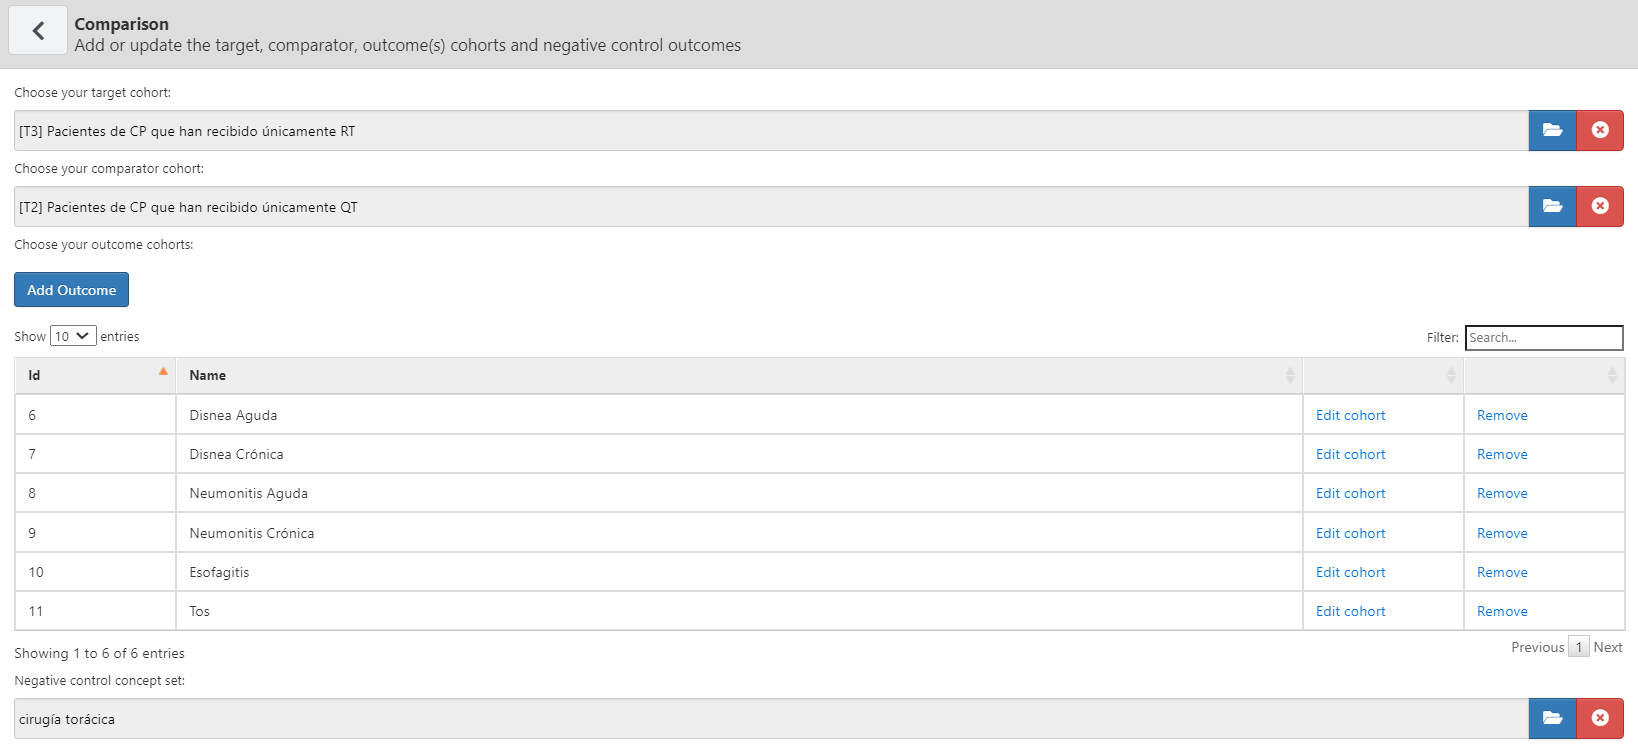
\includegraphics[width=1\textwidth]{figures/comparisonPLE.png}
    \caption{Ajustes de la comparación para la estimación a nivel de población en ATLAS}
    \label{figure:comparisonPLE}
\end{figure}

Para configurar los ajustes del análisis se han seguido las recomendaciones del capítulo 12 ''Population-Level Estimation'' del Libro de OHDSI \parencite{OHDSIbook}, correspondientes con los ajustes establecidos por defecto por la propia herramienta ATLAS. 

\begin{figure}[H]
    \centering
    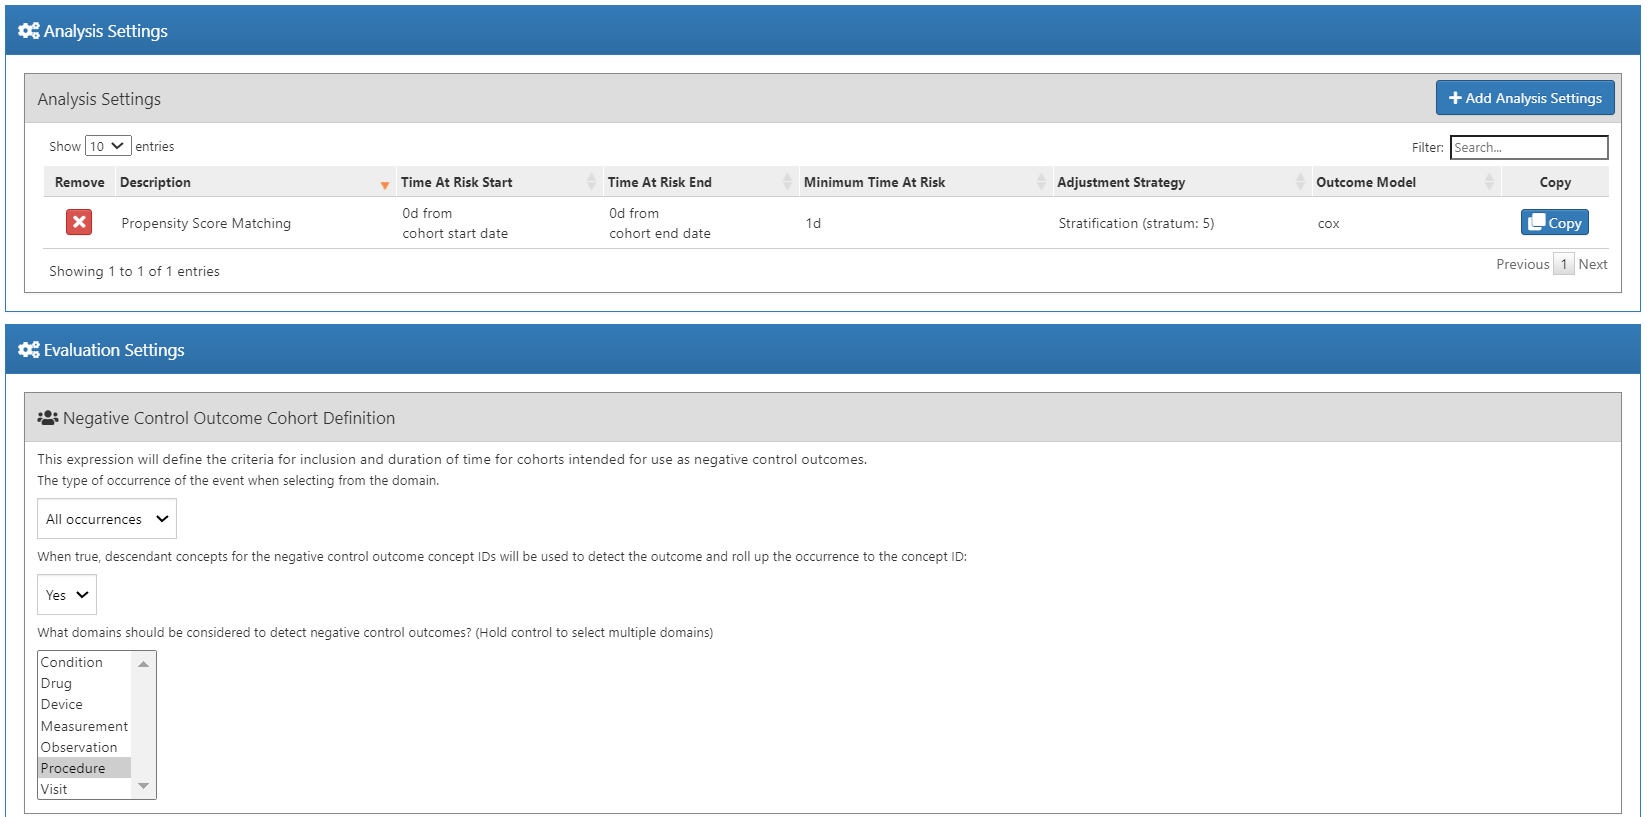
\includegraphics[width=1\textwidth]{figures/ajustesPLE.png}
    \caption{Ajustes predeterminados para la estimación a nivel de población en ATLAS}
    \label{figure:ajustesPLE}
\end{figure}


Una vez que se define el estudio se genera un paquete R para ejecutar el estudio en un entorno de programación más avanzado.\textbf{ La tarea de ATLAS no es realizar este tipo de estudios sino estandarizar la forma de definirlos}. Dicho paquete está disponible en el repositorio de github en la ruta \code{Thesis-ATLAS-OHDSI/atlas/estimation}.


\subsubsection{Predicción a Nivel de Paciente}

Por último en este caso, el estudio realizado por el HUVR correspondía concretamente a una predicción a nivel de paciente, tal y como se justifica en apartados anteriores. Esta tarea en ATLAS se realiza a través del menú \code{Prediction}

Se pretende estudiar la probabilidad de experimentar alguno de los seis efectos adversos (DA, DC, NA, NC, T, E) en los pacientes que reciben tratamiento radioterápico o quimioterápico indistintivamente sin haber sufrido cirugía torácica (cohorte T4).

A continuación se muestra la definición del problema de predicción mediante la interfaz gráfica de ATLAS.

\begin{figure}[H]
    \centering
    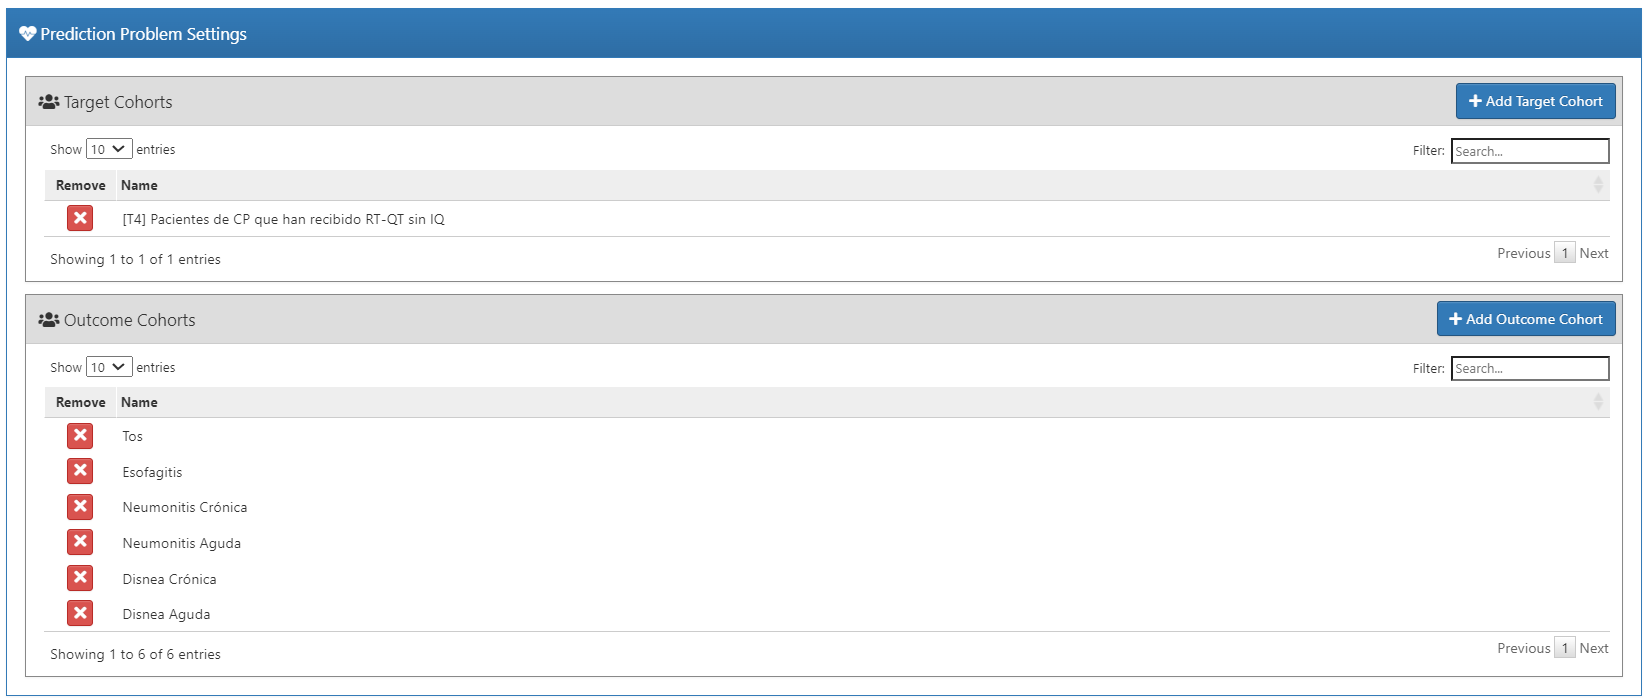
\includegraphics[width=1\textwidth]{figures/predictionPLP.png}
    \caption{Ajustes para la predicción a nivel de paciente en ATLAS}
    \label{figure:predictionPLP}
\end{figure}

De nuevo, una vez que se define el estudio se genera un paquete R para ejecutar el estudio en un entorno de programación más avanzado debido a que la tarea de ATLAS no es realizar este tipo de estudios sino estandarizar la forma de definirlos. Dicho paquete está disponible en el repositorio de github en la ruta \code{Thesis-ATLAS-OHDSI/atlas/prediction}

\subsection{Resultados}

Los resultados del estudio son algo limitados porque no se pueden ejecutar la mayoría de los análisis debido a que la base de datos no contiene la información sobre los efectos adversos y los estudios giran alrededor de la caracterización, estimación o predicción de estos efectos en las cohortes. A continuación se listan algunos resultados:

\begin{itemize}
    \item \textbf{Posibilidad de diseñar el estudio sin poseer los datos.} Es destacable y de gran interés la facilidad que proporciona ATLAS para diseñar estudios precisamente sin disponer de los datos exactos, como es este caso. Gracias a la abstracción lógica de los datos mediante los grupos de conceptos y cohortes, se pueden diseñar los estudios sin necesidad de manipular los datos subyacentes. Esto es también un beneficio a la hora de realizar los estudios en diferentes bases de datos.
    
    De hecho, si Eunomia (la base por defecto de ATLAS Broadsea) incluyese información oncológica, se podrían ejecutar los estudios a la vez sobre las dos bases de datos y comparar resultados de una forma muy sencilla.

    \item \textbf{Reproducibilidad del estudio.} También, como se ha mencionado durante la metodología, los resultados más destacables son la cantidad de archivos exportables que genera ATLAS con la finalidad de favorecer la reproducibilida del estudio. Prácticamente cada paso que se da durante el diseño del estudio en ATLAS es exportable, y de igual forma importable, permitiendo el intercambio de información entre sistemas e investigadores.

    \item \textbf{Limitación en la ejecución del estudio.} No se obtienen resultados tangibles o concretos sobre la estimación o la predicción porque no se llegan a ejecutar estos estudios en el entorno R, debido a la carencia de la base de datos y a que su ejecución se puede considerar fuera del alcance del proyecto, si bien se definía anteriormente que el objetivo del estudio no es reproducirlo sino estandarizarlo. En clave de estandarización se ha demostrado que ATLAS es una herramienta muy poderosa para realizar esta tarea mediante una interfaz muy intuitiva y fácil de usar.
    
\end{itemize}

\section{Discusión de resultados} \label{sec:09resultados}

Volviendo al objetivo inicial del estudio, a la hora de facilitar y apoyar la toma de decisiones durante la planificación radioterápica en pacientes oncológicos, ambos estudios podrían proporcionar resultados muy positivos. 

Si bien es verdad que no se ha podido ejecutar completamente el estudio diseñado en ATLAS por las limitaciones encontradas, en mi opinión en este caso no es un factor que haya impedido demostrar que la herramienta está más que preparada para apoyar la decisión clínica y realiza dicha tarea de forma más beneficiosa que la programación directamente sobre un script de código, tal y como se presentaba en la sección \ref{subsec:05vias} ''Vías de implementación del análisis''. 

Una característica fundamental para ello que sí se ve reflejada durante el análisis es la interfaz gráfica intuitiva y las facilidades que proporciona la herramienta para conducir cualquier estudio. El hecho de que ATLAS sea \textit{low-code} y esté estructurado de una forma preestablecida favorece la conducción del estudio según las opciones pre-establecidas de la herramienta, siendo esto mucho más fácil que enfrentarse directamente a un script de código en blanco, aparte de los beneficios en términos de estandarización del análisis que conlleva.

También aporta el beneficio de poder exportar el código subyacente a la herramienta, de modo que una tarea tan compleja a nivel de conocimiento informático como programar un problema de predicción o estimación mediante técnicas de Machine Learning, queda simplificado a un \textit{''juego''} de combinar cohortes y parámetros de análisis. ATLAS permite programar sin saber programar y eso es una ventaja absoluta sobre cualquier otra herramienta.

Al fin y al cabo, si el objetivo es ayudar al diagnóstico médico se debe tener en cuenta que el doctor no tiene por qué poseer conocimientos informáticos. Sería más fácil para un doctor entender ATLAS que aprender a programar en python o R. Por tanto, ATLAS puede favorecer también el interés por el análisis de datos en profesionales cuyos conocimientos informáticos sean más limitados pero quizás sus conocimientos clínicos sean más profundos, favoreciendo también la investigación clínica de esta forma. 


\section{Conclusiones} \label{sec:09conclusiones}

%A modo de conclusión se incide en la importancia de ATLAS en la estandarización de los sistemas de informática clínica y la relevancia de su configuración \textit{low-code} para democratizar la aplicación de esta tarea en la investigación clínica observacional. También se destaca la importancia de las guías de buenas prácticas para conducir estudios, como ha sido el Libro de OHDSI a la hora de realizar el estudio con ATLAS, permitiendo a investigadores sin experiencia conducir estudios informáticos complejos.

ATLAS es fundamental para la estandarización de los sistemas de informática clínica, mejorando la interoperabilidad y la calidad de la investigación. Su configuración \textit{low-code} democratiza la investigación clínica observacional, permitiendo que profesionales sin conocimientos avanzados en programación participen en estudios complejos. Además, las guías del Libro de OHDSI son cruciales para realizar estudios rigurosos y reproducibles, permitiendo a investigadores sin experiencia informática llevar a cabo investigaciones de alta calidad, elevando la credibilidad y validez científica.

%- Importancia de la estandarizacion y relevancia del lowcode

%- Buenas practias e.g IMPACT DATA